\chapter{}

\section{Screen Shot}
\paragraph{}
Figures~\ref{fig:d1} and~\ref{fig:d2} show the original dashboard (ingestion overview with ground-truth confusion matrix, and the threat-alert forensics table). The \emph{Batch Lake Analytics} and \emph{System Health \& Disaster Recovery} tabs added in this work are described in Section~7.5 and can be reproduced with \texttt{docs/DEMO\_GUIDE.md}.

\begin{figure}[H]
\centering
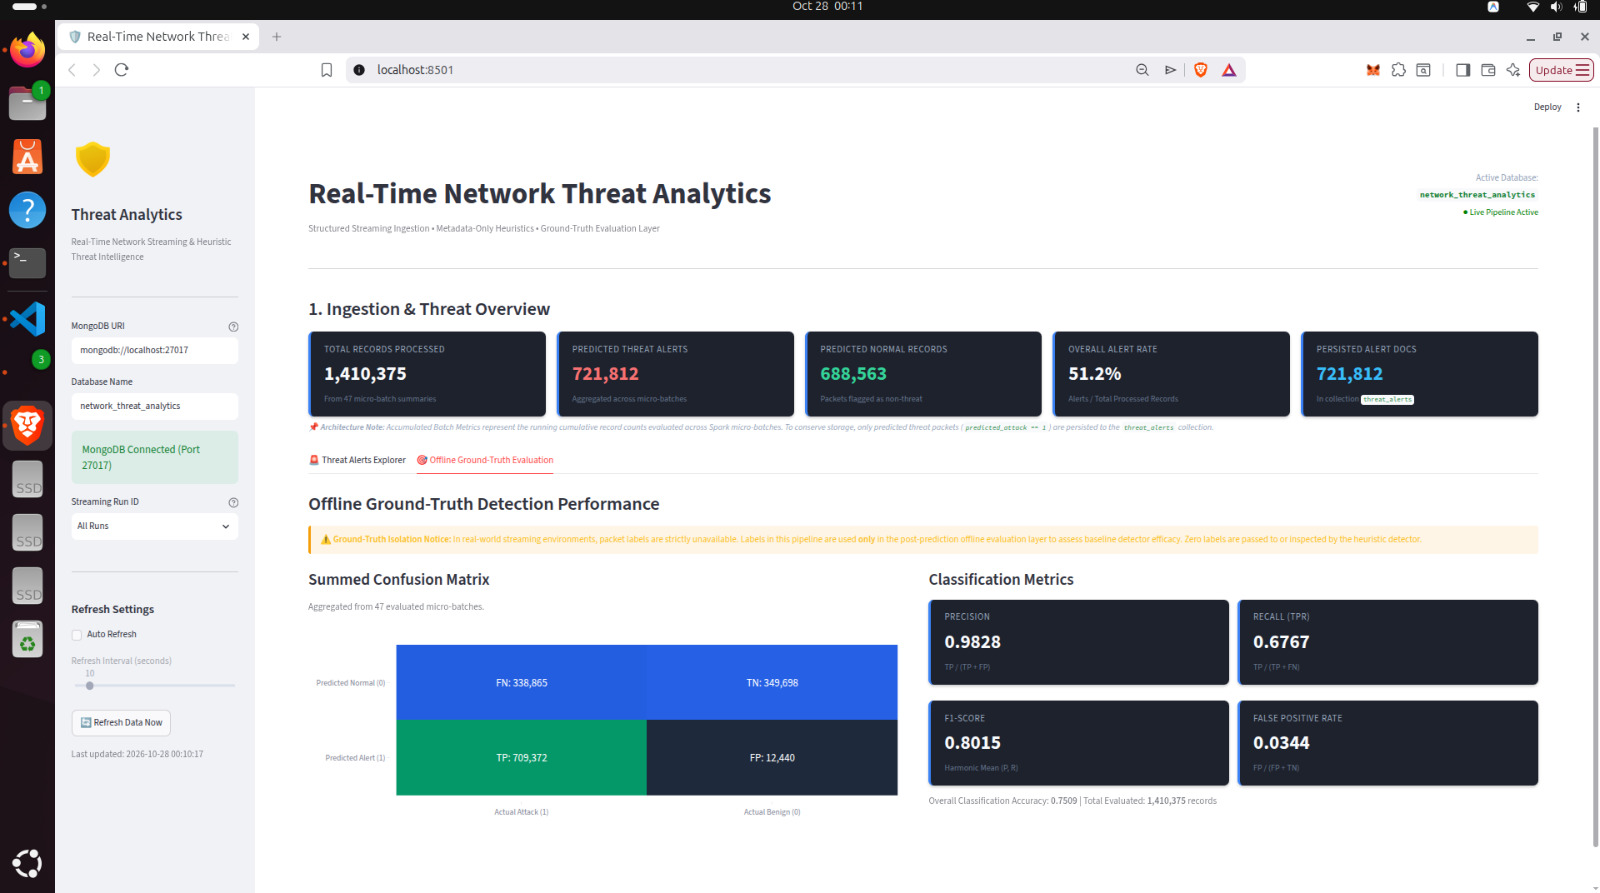
\includegraphics[width=\textwidth]{images/ScreenShots/Dashboard1.jpeg}
\caption{Dashboard: ingestion overview and confusion matrix}\label{fig:d1}
\end{figure}
\begin{figure}[H]
\centering
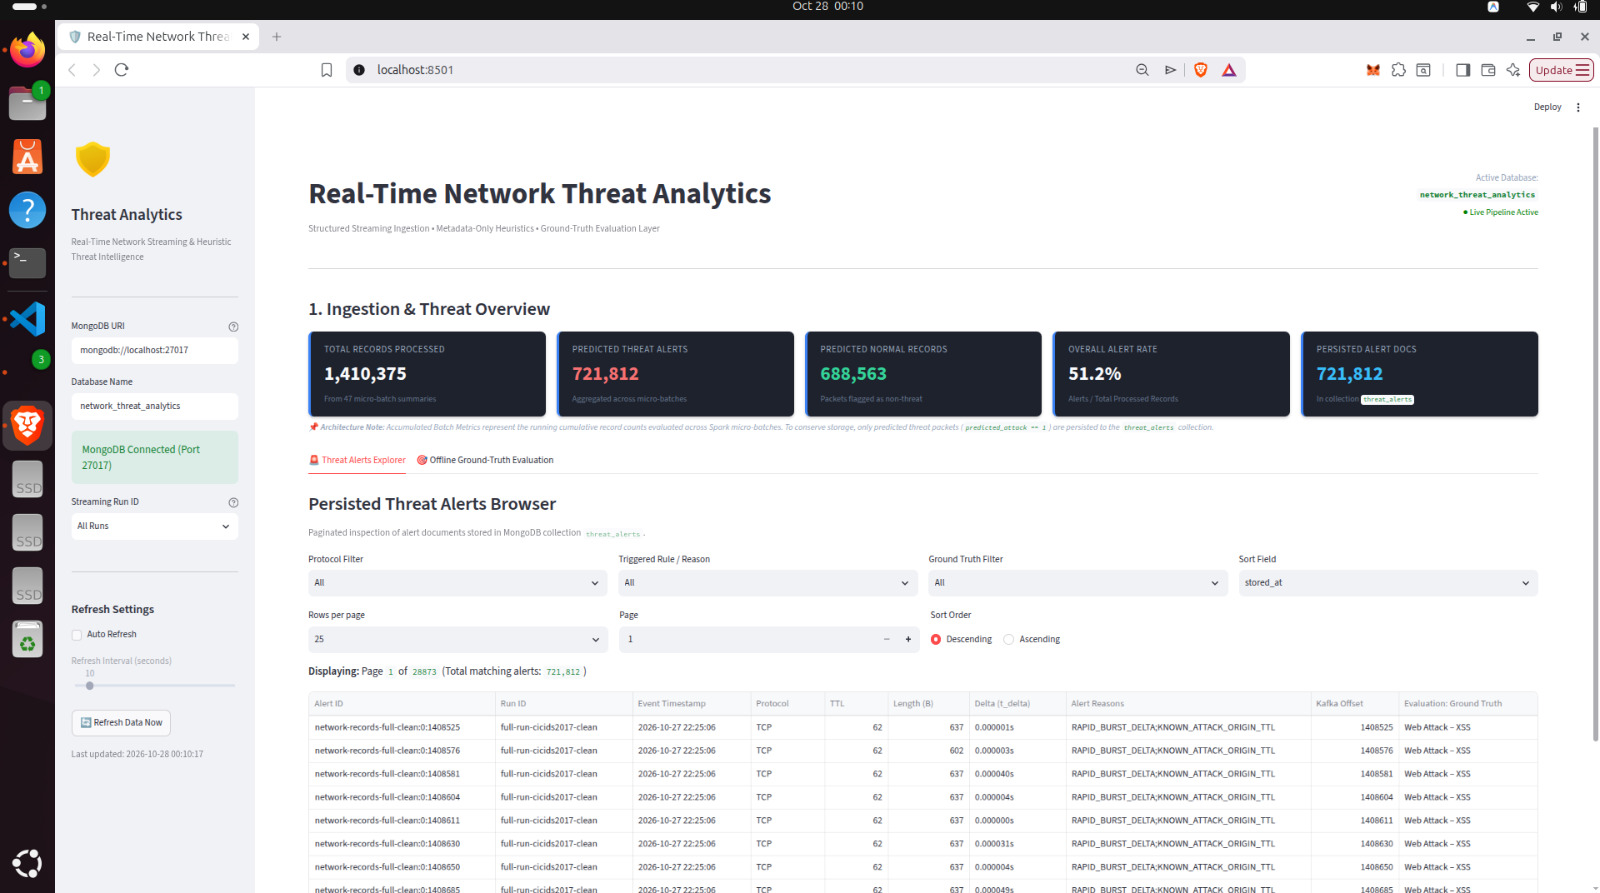
\includegraphics[width=\textwidth]{images/ScreenShots/Dashboard2.jpeg}
\caption{Dashboard: threat alerts explorer}\label{fig:d2}
\end{figure}

\section {Gantt Chart}
\paragraph{}
% TODO: insert the team's Gantt chart (not generated automatically).
To be added by the team.

\section {Glossary}
\begin{description}[noitemsep]
\item[Shard] A horizontal partition of a collection stored on one replica set.
\item[Shard key] The field(s) that decide which shard owns a document.
\item[Replica set] A primary and secondaries holding copies of the same data; a new primary is elected when the primary fails.
\item[mongos] The router that sends client operations to the correct shard(s).
\item[Lambda architecture] Speed layer, batch layer and serving layer over an immutable master dataset.
\item[RPO / RTO] Recovery point objective (data that may be lost) and recovery time objective (time to restore).
\item[Micro-batch] A small set of stream records processed together by Spark Structured Streaming.
\item[Parquet] A columnar, compressed file format.
\end{description}

\section {Description of Tools and Technology used}
\paragraph{}
Apache Kafka 4.3.1 (KRaft), Apache Spark 3.5.6 (Structured Streaming, MLlib, SQL), MongoDB 8.0.4 (sharded cluster, database tools), Apache Parquet with Snappy, Python 3.11 (kafka-python, pymongo, pyarrow, pandas), Streamlit and Plotly, OpenJDK 17, Ubuntu 26.04.

\section{Blue Print}
Attach your Blue Print file at the end

\section{Plagiarism Report}
Attach your Plagiarism Report file at the end
